\begin{frame}\frametitle{Background}
\begin{Large}
Background
\end{Large}
\begin{enumerate}
\item Skip Gram Model 
\item Skip Gram with Negative Sampling (SGNS)
\end{enumerate}
\end{frame}
\begin{frame}\frametitle{Background}
Main idea: train a network on a "fake task" then use the weights as embedding. \bigskip
\begin{itemize}
\item The fake task:
\item Given a word $w$ guess the context words. 
%\item We want to maximize the following probability:
\end{itemize}
%\begin{equation}
%\prod_{t=1}^T \prod_{-m<j<m}  p(w_{t+j}|w_t)
%\end{equation}
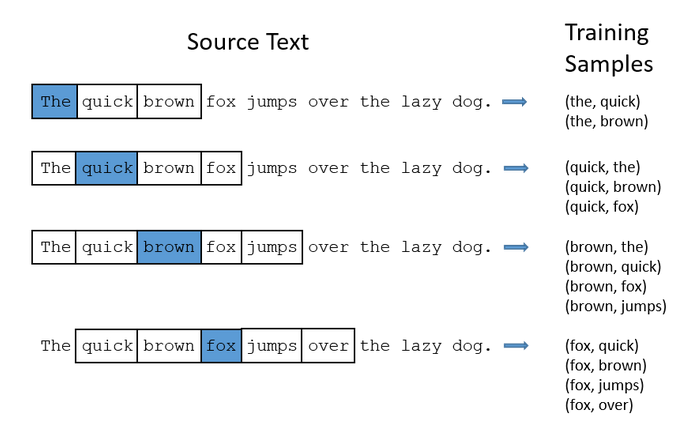
\includegraphics[scale=0.37]{images/context_pairs.png}
\end{frame}

\begin{frame}\frametitle{Background}\framesubtitle{Network achitecture}
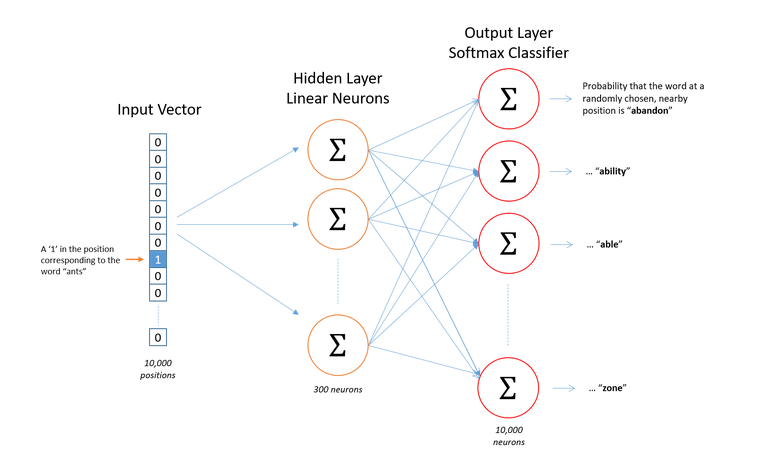
\includegraphics[scale=0.37]{images/ntw_architecture.png}
(Source: http://mccormickml.com/2016/04/19/word2vec-tutorial-the-skip-gram-model/) 
\end{frame}
\iffalse
\begin{frame}\frametitle{Background}\framesubtitle{Example}
$
\newcolumntype{g}{>{\columncolor{green! 20}}c}
\newcolumntype{b}{>{\columncolor{blue! 20}}c}
\newcolumntype{r}{>{\columncolor{red! 20}}c}
\left(
\begin{array}{cbc}
0 & 1 & 0 
\end{array}\right)
\left(
\begin{array}{ccc}
\rowcolor{green! 20}
1 & 1 & 1  \\
\rowcolor{blue! 20}
2 & 2 & 2 \\
\rowcolor{red! 20}
3 & 3 & 3 \\
\end{array}\right)
= 
\left(
\begin{array}{ccc}
\rowcolor{blue! 20}
2& 2 & 2
\end{array}\right)
\newcolumntype{g}{>{\columncolor{green! 20}}c}
\newcolumntype{b}{>{\columncolor{blue! 20}}c}
\newcolumntype{r}{>{\columncolor{red! 20}}c}
\left(
\begin{array}{gbr}
0.1 & 0.2&0.3  \\
0.1 & 0.2&0.3  \\
0.1 & 0.2&0.3 \\
\end{array}\right)
$
$
= 
\newcolumntype{g}{>{\columncolor{green! 20}}c}
\newcolumntype{b}{>{\columncolor{blue! 20}}c}
\newcolumntype{r}{>{\columncolor{red! 20}}c}
\left(
\begin{array}{gbr}
0.6 & 1.5 & 3 
\end{array}\right)
\implies Softmax:
\left(
\begin{array}{gbr}
0.13 & 0.31 & 0.56 
\end{array}\right)
$
$
c
$
\vspace{10pt}

$
p(v_{he}| v_{is})   
 $
 
 \vspace{10pt}
 
 $
 p(v_{king}| v_{is})
 $

\end{frame}
\fi

\begin{frame}\frametitle{Background}
   \begin{flalign}
\text{Softmax: } &&  p(c|w) =  \frac{exp( {v^{'}_c}^\intercal v_w )}{\sum_{i=1}^T exp({v^{'}_i}^\intercal v_{w})}
   \end{flalign}
  \hfill   $v^{'} $is the output layer vector
  $v$ is the input layer vector
\begin{large}
Negative Sampling
\end{large}
\begin{itemize}
\item Distinguish data from noise $\Rightarrow$ reduce problem to a logistic regression. 
\item Guess k random samples 
\item For each pair $(w,c)$ we get:
\medskip
\end{itemize}
  \begin{flalign}
 && \argmax_{\theta }\ log(\sigma({v^{'}_c}^\intercal v_w ) + \sum_{k\in K} log(\sigma(-{v^{'}_k}^\intercal  v_w ))  
  \end{flalign}
  \begin{itemize}
  \item Uses SGD as an optimizer
  \end{itemize}
\end{frame}

\begin{frame}
\frametitle{Background}
\begin{Large}
State of the Art
\end{Large}
\begin{itemize}
\item word2vec (Mikolov et al. 2013)  \cite{mikolov}
\item Parallelizing Word2Vec in Shared and Distributed Memory (Ji et al. 2016)\cite{intel}
\item Acceleration of Word2vec Using GPUs (Seulki and Youngmin  2016) \cite{gpu}
\item Gensim ({\v R}eh{\r u}{\v r}ek and Sojka) \cite{gensim}
\end{itemize}
\begin{Large}
Research Questions:
\end{Large}
\medskip \\
 Can the convergence time of the skip Gram Model be optimized by the use of:
\begin{itemize}
\item Advanced optimizers
\end{itemize}
and
\begin{itemize}
\item Input Shuffling
\end{itemize}
while at the same time maintaining it's accuracy? 
\end{frame}